\section{Networking}\lecture[4 hours]{28}{05}{2024}\lecture[4 hours]{29}{05}{2024}
\subsection{Network Categories: Geographical and Topological}
\subsubsection{Geographical Networks}

Networks can be categorized based on the geographical distance between devices. The primary types of geographical networks include:

\paragraph{WAN - Wide Area Network}
Wide Area Networks (WANs) connect computers over large distances, covering extensive geographical areas. WANs use various transmission methods such as satellites, fiber optics, and cables. The quintessential example of a WAN is the Internet, which allows computers in different continents to communicate within seconds.

\paragraph{LAN - Local Area Network}
Local Area Networks (LANs) connect computers within a smaller geographical area, such as the floors of a building in a company. LANs are popular due to their high speed and relative ease of installation.

\paragraph{PAN - Personal Area Network}
Personal Area Networks (PANs) cover very limited areas, such as the connection between a mobile phone and a computer.

\subsubsection{Topological Networks}

Networks can also be categorized based on their physical configuration. The primary types of topological networks include the following, also shown in \Cref{fig:net_topo}.

\begin{figure}[h]
    \centering
    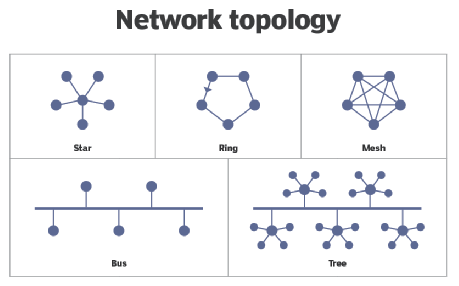
\includegraphics[width=\textwidth]{images/network_topology.png}
    \caption{Network topologies.}
    \label{fig:net_topo}
\end{figure}

\paragraph{Bus Topology}
In a bus topology, devices share a single transmission channel, typically a single cable. One of the advantages of bus topology is its simplicity and ease of implementation.

\paragraph{Ring Topology}
In a ring topology, devices are connected in a circular manner. These networks are more complex and expensive than bus networks and are generally used in enterprise environments for corporate LANs.

\paragraph{Star Topology}
In a star topology, devices are individually connected to a central device, such as a switch or router, using dedicated cables or other physical media. Each computer has a dedicated link to the central device and can communicate with other devices through it. Star networks are the most widely used due to their performance and security characteristics.

Understanding the different types of networks, both geographical and topological, is essential for designing and implementing efficient and secure network infrastructures. WANs, LANs, and PANs cater to different geographical scopes, while bus, ring, and star topologies offer various configurations to meet specific organizational needs.


\subsection{Basic Networking Concepts}

A computer network enables and facilitates communication between people, applications, and servers regardless of their geographical location. The Internet is the largest example of a computer network that we use on a daily basis. In a computer network, machines communicate with each other using communication \textit{protocols}, which ensure communication between computers with different hardware and software.

\subsubsection{Data Transmission}

Communication occurs through an exchange of data, or information, which is transported in the form of \textit{packets}. Packets are streams of bits exchanged via electrical signals over a physical medium. The physical medium can be a LAN (local area network) cable or, very commonly, the air in a Wi-Fi network.

\begin{figure}[h]
    \centering
    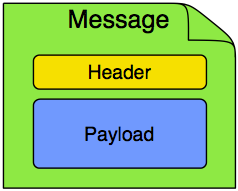
\includegraphics[width=0.4\textwidth]{images/message.png}
    \caption{Structure of a Packet: Header and Payload.}
    \label{fig:packet_structure}
\end{figure}

\subsubsection{Packet Structure}

A \textit{packet} has a defined structure as shown in \Cref{fig:packet_structure}. The \textit{Header} depends on the protocol used in the communication. Its task is to ensure that the receiving computer can interpret the \textit{Payload} and manage the communication. The \textit{Payload}, on the other hand, is the actual information. For instance, it could be a message, or part of a message sent from one computer to another, an email, or other data.

\subsection{The ISO/OSI Model}

To standardize network communication, in 1984 the International Organization for Standardization (ISO) published a theoretical model subsequently called the \textit{Open System Interconnection (OSI)} model. The ISO/OSI model is used as a theoretical reference. It is based on a stack of 7 layers, also called \textit{layers}, where each layer serves the upper layer and has exclusive protocols.

\begin{figure}[h]
    \centering
    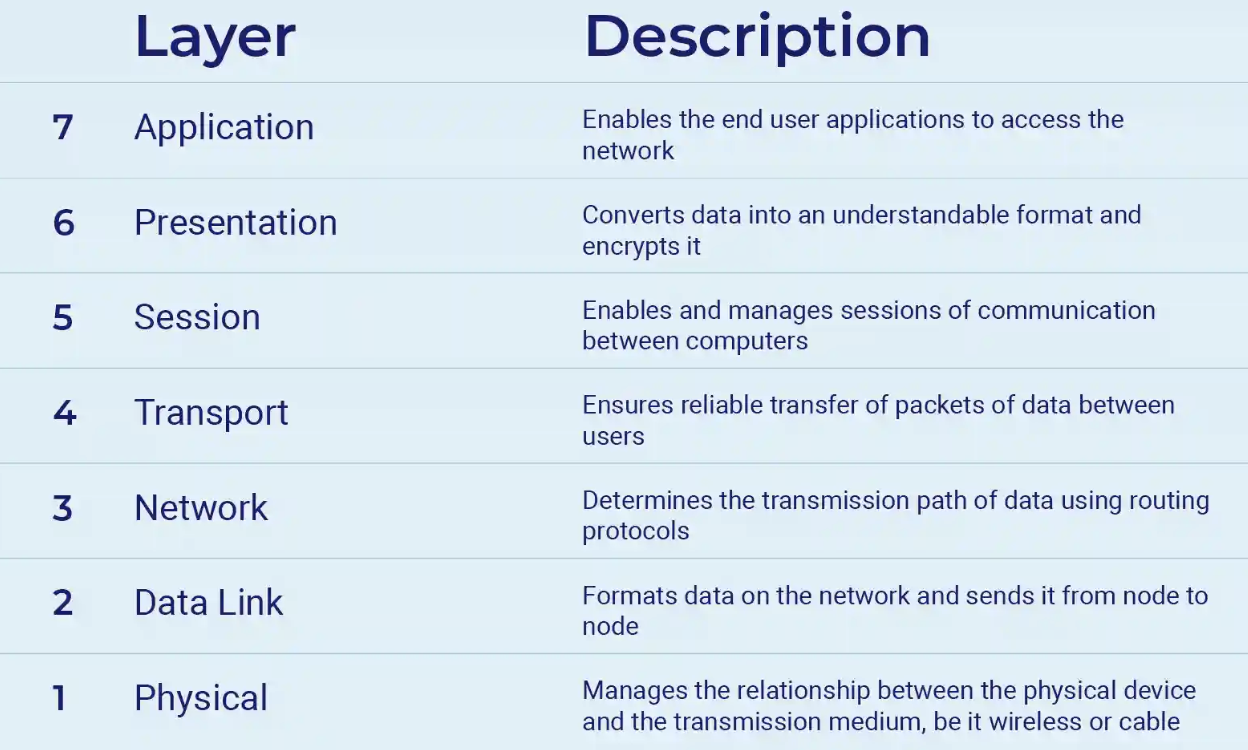
\includegraphics[width=\textwidth]{images/layers_osi.png}
    \caption{The ISO/OSI Model Layers.}
    \label{fig:osi_layers}
\end{figure}

In a communication between two computers, the data follows the logical model as represented by the line in \Cref{fig:osi_model}.

\begin{figure}[h!]
    \centering
    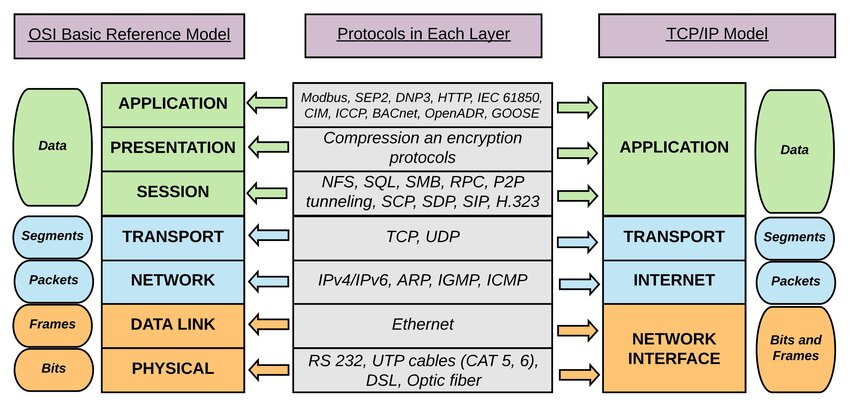
\includegraphics[width=\textwidth]{images/iso_osi_tcp.png}
    \caption{The ISO/OSI vs TCP/IP model.}
    \label{fig:osi_model}
\end{figure}

Note that the ISO/OSI model is a theoretical model to be used as a reference. In practice, applications use the \textit{TCP/IP} model, which slightly varies from the theoretical ISO/OSI model.

The differences between TCP/IP and the ISO/OSI model are depicted in \Cref{fig:osi_model} and summarized in \Cref{fig:tcp_vs_osi}. For theoretical study of concepts, we will follow the notions of the ISO/OSI model.

\begin{figure}[h!]
    \centering
    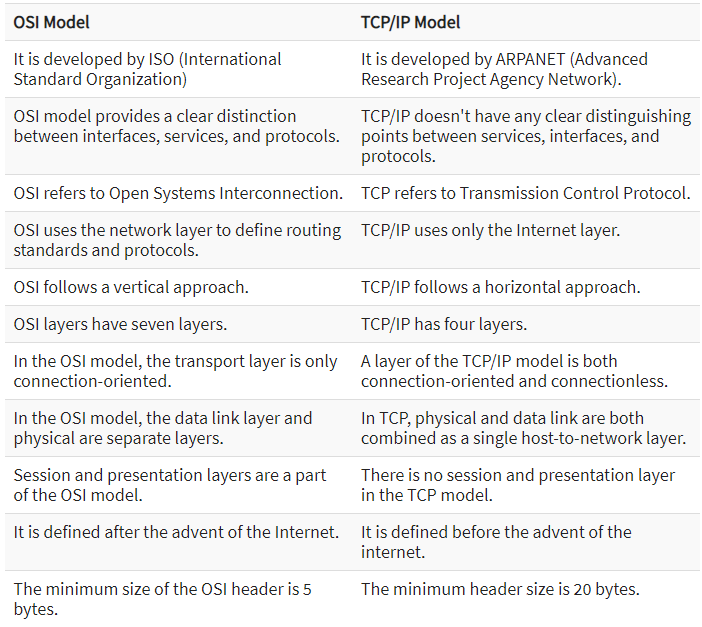
\includegraphics[width=\textwidth]{images/tcp_vs_osi.png}
    \caption{The ISO/OSI vs TCP/IP model.}
    \label{fig:tcp_vs_osi}
\end{figure}


\subsubsection{\textbf{Physical Layer}}
The physical layer is responsible for the transmission of raw data bits over a physical medium. This transmission can occur via various types of cabling, such as copper wires or fiber optics. Data from higher layers of the source computer is segmented and sent to the physical layer of the receiving computer in the form of bits.

\paragraph{Bits and Binary System}
The bit, short for binary digit, is the basic unit of information in computing, represented as either '0' or '1'. Unlike the decimal system, which uses ten digits (0-9), computers operate using the binary system. Consequently, information is transmitted over a physical cable as a sequence of binary digits, for example, 10010010 10011110, etc.

\subsubsection{\textbf{Data Link Layer}}
The Data Link Layer utilizes the services of the physical layer to send and receive bits over communication channels. Packets at this layer are referred to as frames. The main functions of the Data Link Layer include:

\begin{itemize}
    \item Providing an interface to the Network Layer (Layer 3)
    \item Handling transmission errors
    \item Regulating the flow of bits between two communicating devices
\end{itemize}

The Data Link Layer plays a crucial role by defining protocol standards such as IEEE 802.3 for Ethernet (wired connections) and IEEE 802.11 for Wireless connections.

\paragraph{MAC Address}
In a computer network, two personal computers communicate at the Data Link Layer using what is called a physical address or more commonly, a MAC Address. The MAC address is a 48-bit identifier typically represented in hexadecimal format. Below is a table showing the conversion between binary and hexadecimal systems:

\begin{table}[h]
    \centering
    \begin{tabular}{|c|c|}
        \hline
        \textbf{Binary} & \textbf{Hexadecimal} \\
        \hline
        0000 & 0 \\
        0001 & 1 \\
        0010 & 2 \\
        0011 & 3 \\
        0100 & 4 \\
        0101 & 5 \\
        0110 & 6 \\
        0111 & 7 \\
        1000 & 8 \\
        1001 & 9 \\
        1010 & A \\
        1011 & B \\
        1100 & C \\
        1101 & D \\
        1110 & E \\
        1111 & F \\
        \hline
    \end{tabular}
    \caption{Binary to Hexadecimal Conversion}
    \label{tab:bin_hex}
\end{table}

An example of a MAC Address is 00:AA:11:BB:22:CC. The MAC address is a unique identifier assigned to the network interfaces of devices.

\paragraph{Ethernet Frame Structure}
The structure of an Ethernet 802.3 frame includes fields for the Destination MAC Address and the Source MAC Address. These fields are automatically populated with the MAC addresses of the source and destination when an exchange of information begins at the Data Link Layer.

\paragraph{Role of Switches}
Switches are vital network devices for communication but come with certain disadvantages. They route broadcast packets across the entire network. Broadcast packets are sent to a specific MAC address, FF:FF:FF:FF:FF:FF, which is received by the switch and routed to all nodes connected to it. This creates what is known as a broadcast domain.

A broadcast domain includes all the devices on a network segment that receive broadcast frames from any device within the segment. In a large network with numerous devices, this can cause significant latency issues.

\paragraph{Address Resolution Protocol (ARP)}
ARP, or Address Resolution Protocol, is a network protocol used to map IP addresses to MAC addresses within a local network. Its primary functions include:

\begin{itemize}
    \item \textbf{ARP Request}: A device broadcasts an ARP request on the local network, asking for the MAC address associated with a specific IP address.
    \item \textbf{ARP Reply}: The destination device responds with a packet containing its MAC address associated with the requested IP address.
    \item \textbf{ARP Cache}: Devices maintain an ARP table or ARP cache that stores IP-to-MAC address mappings.
\end{itemize}


ARP is crucial for communication within the same local network. When a device needs to send data to another device within the same subnet, it uses ARP to discover the MAC address corresponding to the destination IP address.

\paragraph{Virtual LAN (VLAN)}\lecture[4 hours]{30}{05}{2024}
Switches allow the segmentation of broadcast domains through the creation of Virtual LANs (VLANs). A VLAN is a logical grouping of hosts and network devices. VLANs are created by adding a "tag" or VLAN ID to the switch ports, or by mapping the MAC address of the host to the VLAN ID.

Assume we want to restrict communication and the broadcast domain to hosts A, B, and C. We create a VLAN identified by ID 100 and associate the MAC addresses of hosts A, B, and C with that VLAN.

When host A sends a packet to the broadcast address, it will only be received by hosts B and C. Therefore, VLANs segment broadcast domains and eliminate latency issues in large networks.


VLANs are essential for managing broadcast domains within a network. By associating specific MAC addresses with VLAN IDs, we can ensure that broadcast traffic is limited to only those hosts within the same VLAN, thus improving network efficiency and reducing latency.


\subsubsection{\textbf{Network Layer}}
In networking, just as there are specific devices at the Data Link Layer that facilitate communication between personal computers on the same network, there are devices at the Network Layer, such as router-gateways, that enable data routing between personal computers connected to different networks. For instance, consider the following network configuration:

\paragraph{Role of the Router}
A switch operates at Layer 2 and does not route packets to other networks because it forwards packets based on MAC addresses rather than IP addresses. The solution is to use a Layer 3 device like a router-gateway.

The router receives the packet from the switch and checks its routing table to determine which of its interfaces to forward the packet to reach the destination network.

\paragraph{Example of Router Operation}
To better understand how a router-gateway functions, consider a router connected with three interfaces to three different networks:

If a personal computer on network $2.228.1.0$ wants to send a packet to a PC on network $2.175.1.0$, the packet will be sent to the router, which will check its routing table to see which interface to use to forward the packet.

In a network, computers interact using both MAC and IP addresses. For example, if PC A wants to send a packet to PC B, it will structure the packet as follows:

\begin{itemize}
    \item The destination IP address of B in the datagram header (Layer 3).
    \item The MAC address of the router as the destination in the frame header (Layer 2). The router, in this case, is the "next hop."
    \item Its IP address as the source in the datagram header.
    \item Its MAC address as the source in the frame header.
\end{itemize}

The router will receive the packet and set:
\begin{itemize}
    \item The destination MAC address to that of B.
    \item The source MAC address to that of its corresponding interface.
\end{itemize}

Routers play a crucial role in network communication by enabling the routing of data between different subnets. This process involves intricate interactions between Layer 2 (MAC addresses) and Layer 3 (IP addresses) addressing schemes, ensuring seamless communication across diverse network segments.

\subsubsection{\textbf{Transport Layer}}
The transport layer, also known as layer 4 in the OSI model, is responsible for establishing a logical connection or channel between applications on different computers. It ensures the reliable transmission of data packets between a source and a destination. Packets may get lost during transmission due to network congestion, communication errors, or network issues. In some scenarios, minor transmission issues are tolerable, such as in phone conversations or video streaming, where a lost packet might result in a brief glitch. However, for activities like financial transactions or logging into a portal, it's crucial that communication is lossless.

\paragraph{Protocols in the Transport Layer}
The transport layer provides two fundamental protocols for communication between hosts:
\begin{itemize}
    \item \textbf{TCP (Transmission Control Protocol)}: TCP guarantees data traffic control and reliable delivery to the recipient, making it more secure for applications requiring guaranteed packet delivery. The reliability of TCP is due to its connection-oriented nature, which establishes a communication channel before data exchange. TCP follows a three-step process called the \textit{three-way handshake} to establish this connection.
    \begin{enumerate}
        \item The client initiating the connection sends a TCP packet with the SYN flag set and a random sequence number.
        \item The server responds with a packet that has both SYN and ACK flags set, along with its own sequence number and an acknowledgment number equal to the client's sequence number plus one.
        \item The client completes the synchronization by sending a packet with the ACK flag set, acknowledging the server's sequence number.
    \end{enumerate}
    \item \textbf{UDP (User Datagram Protocol)}: UDP is a connectionless protocol that does not require establishing a communication channel before data exchange. It is more lightweight and faster, suitable for activities requiring data streaming (e.g., video or audio). However, it does not guarantee packet delivery.
\end{itemize}


\paragraph{Ports and Services}
To identify the target process or service for a given packet, both TCP and UDP use ports, represented as \texttt{<ip>:<port>}. While the IP identifies the destination machine, the port provides information about the service. Ports can be categorized into:

\begin{itemize}
    \item \textbf{Well-known ports}: Used for standard services, ranging from 0 to 1023.
    \item \textbf{High ports}: Used for non-standard services, ranging from 1024 to 65535.
\end{itemize}

\begin{table}[h]
    \centering
    \begin{tabular}{|c|c|}
        \hline
        \textbf{Protocol} & \textbf{Port} \\
        \hline
        SMTP & 25 \\
        SFTP & 115 \\
        HTTP & 80 \\
        HTTPS & 443 \\
        SSH & 22 \\
        Telnet & 23 \\
        POP3 & 110 \\
        FTP & 21 \\
        \hline
    \end{tabular}
    \caption{Commonly Used Ports}
    \label{tab:ports}
\end{table}

Understanding the transport layer is crucial for ensuring reliable communication between applications on different hosts. TCP and UDP provide different levels of service, making them suitable for various applications. TCP's connection-oriented nature and reliable delivery make it ideal for critical applications, while UDP's connectionless nature and speed make it suitable for real-time data streaming.


\subsubsection{\textbf{Session Layer}}
In order to enable communication between two hosts, or between a client and a server, it is necessary to first establish a session. This is precisely the role of the protocols that are part of the session layer. Sessions are essential to ensure the correct transfer of information. It is very important to define the rules for opening, closing, or maintaining a session. We can identify two main purposes of the session layer:

\begin{itemize}
    \item Definition and management of the session:
    \begin{itemize}
        \item \textbf{Initiating or opening a session} between a user who intends to use a service that is listening on a specific server. A common example is the \textit{SSH} (Secure Shell) protocol, which is used by system administrators to create sessions on remote servers.
        \item \textbf{Maintaining the session} for its duration, ensuring the session remains active during the flow of information.
        \item \textbf{Closing the session}, either upon the request of the user or the server.
    \end{itemize}
    \item Synchronization: saving intermediate checkpoints (or synchronization points) during a data flow. This allows for the preservation of information in the event of an abnormal session interruption.
\end{itemize}

\subsubsection{\textbf{Presentation Layer}}
The Presentation Layer is the sixth level in the OSI (Open Systems Interconnection) model. This layer is responsible for the preparation of data in transit between two hosts before it is presented to the users. One of the critical functions of the Presentation Layer is \textbf{data encryption}. In a communication channel, data can transit in one of two ways:

\begin{itemize}
    \item \textbf{In clear text}: Data is transmitted in a visible and readable form to everyone.
    \item \textbf{Encrypted}: Data is encoded such that only authorized parties can view the content.
\end{itemize}

Encryption transforms clear text data into encrypted data using what is known as an \textbf{encryption algorithm}. The primary purpose of encryption is to ensure that the content of the information is available only to specific users, thereby securing the data from potential malicious actors.

The Presentation Layer performs several critical functions, including:

\begin{enumerate}
    \item \textbf{Translation}: This layer translates data between the application layer and the network format. It ensures that data from the sender's application layer can be understood by the receiver's application layer.
    \item \textbf{Data Encryption and Decryption}: As mentioned, encryption is a fundamental aspect of the Presentation Layer. It encodes the data before it is transmitted over the network and decodes it upon arrival.
    \item \textbf{Data Compression}: The Presentation Layer can compress data to reduce the bandwidth needed for transmission. This can lead to faster transmission times and reduced network load.
    \item \textbf{Character Code Translation}: It translates character codes from one coding system to another. For example, it can convert ASCII to EBCDIC.
    \item \textbf{Data Serialization}: This process involves converting complex data structures into a format that can be easily transmitted over the network.
\end{enumerate}

\paragraph{Encryption}
Encryption is a process that involves transforming readable data, known as \textbf{plaintext}, into an unreadable format, known as \textbf{ciphertext}. This transformation uses an algorithm and an encryption key. Only authorized parties who possess the corresponding decryption key can convert the ciphertext back into readable plaintext.

Encryption serves several essential purposes:

\begin{itemize}
    \item \textbf{Confidentiality}: Ensures that data is only accessible to those who have the appropriate decryption key.
    \item \textbf{Integrity}: Protects data from being altered during transmission.
    \item \textbf{Authentication}: Verifies the identities of the communicating parties.
    \item \textbf{Non-repudiation}: Prevents parties from denying the transmission or receipt of data.
\end{itemize}

The Presentation Layer plays a crucial role in ensuring that data is properly encrypted and decrypted, thereby maintaining the security and integrity of the information being transmitted across networks.


\subsubsection{\textbf{Application Layer}}
The application layer is the seventh and final layer of the ISO/OSI model. This layer interacts directly with the applications used by the end user, providing interface services for applications and support for network access. Among the most well-known protocols of the application layer are:

\begin{itemize}
    \item \textbf{HTTP/HTTPS (Hyper Text Transfer Protocol):} This is the main protocol for transmitting information on the web. HTTPS is the secure, encrypted version of HTTP. The protocol operates on a request/response mechanism, typical of the client/server model, where a host requests a resource from a remote web server.

    \item \textbf{DNS (Domain Name System):} This protocol translates domain name requests (e.g., \texttt{www.google.com}) into IP addresses. DNS is a fundamental protocol for the functioning of the internet. A DNS name like \texttt{www.store.google.com} can be divided as follows:
    \begin{itemize}
        \item \texttt{www} - Host
        \item \texttt{store} - Subdomain
        \item \texttt{google} - Domain
        \item \texttt{com} - Top-Level Domain (TLD)
    \end{itemize}
    The resolution of DNS names is handled by DNS resolvers, which are DNS servers generally provided by ISPs (Internet Service Providers), such as Vodafone, TIM, or Wind3. Public DNS servers, like Google's DNS, are also available.

    \item \textbf{FTP (File Transfer Protocol):} This protocol manages the transfer of data between hosts and is based on TCP.

    \item \textbf{DHCP (Dynamic Host Configuration Protocol):} This protocol allows devices on a LAN to receive network configuration automatically. An host connecting to a network where the DHCP service is active will have its IP address and other network information auto-assigned. For example, when you connect to your home network, you likely don't manually assign an IP address to your PC or smartphone. This is because DHCP is typically enabled on private networks for automatic IP assignment.
\end{itemize}

The application layer provides crucial functionalities that directly support user applications and network services. Here are some key points:

\begin{itemize}
    \item \textbf{User Interface Support:} This layer offers services that directly interface with user applications, enabling seamless communication and data transfer over the network.

    \item \textbf{Protocol Implementation:} Protocols at this layer define the rules for communication between different devices and software applications. These protocols include not only HTTP, DNS, FTP, and DHCP but also others like SMTP (Simple Mail Transfer Protocol), POP3 (Post Office Protocol), and IMAP (Internet Message Access Protocol), which are used for email transmission and retrieval.

    \item \textbf{Resource Sharing:} It facilitates resource sharing across the network, such as file transfers, web pages, and email.

    \item \textbf{Network Transparency:} It provides a way for applications to interact with the network in a manner that abstracts the complexities of lower-layer operations, making network interactions more user-friendly and efficient.
\end{itemize}

The application layer is indispensable for ensuring that user applications can operate over the network effectively, providing the necessary protocols and services to support diverse network-based activities.


\subsection{Network Address Translation (NAT)}
Network Address Translation (NAT) is a technology developed to address the exhaustion of IPv4 addresses. Introduced in the 1990s, it delineates the distinction between private and public IP addresses. NAT is typically configured on routers or firewalls.

A public IP address allows devices to access the Internet, whereas private IP addresses are used within local networks (e.g., home or corporate networks) and are not directly accessible from the Internet. There are various types of NAT, but the basic concept involves translating private IP addresses (used within the local network) into one or more public IP addresses.

\subsection{Port Address Translation (PAT)}
Port Address Translation (PAT) is a specific form of NAT. In addition to translating IP addresses, PAT also translates the port numbers of devices within the local network. Ports are 16-bit numbers associated with each connection, and PAT enables multiple devices to share the same public IP address by distinguishing their connections based on port numbers.

For instance, if you have three devices using PAT and sharing the same public IP address, the first device's connection might use port 5000, the second device might use port 5001, and the third device might use port 5002. This allows the router to keep track of which connection belongs to which device on the local network.

In summary, while NAT translates private IP addresses into one or more public IP addresses, PAT goes further by also translating ports. This enables multiple devices to share the same public IP address, distinguishing them based on the ports used. Both technologies are fundamental for managing the scarcity of public IP addresses and enabling Internet connectivity for multiple devices within a local network.

\paragraph{Private IP Address Ranges}
The following table lists the ranges of IP addresses defined as "private." These IP addresses are assigned only within private networks and are not exposed or reachable via the Internet.

\begin{figure}[h!]
    \centering
    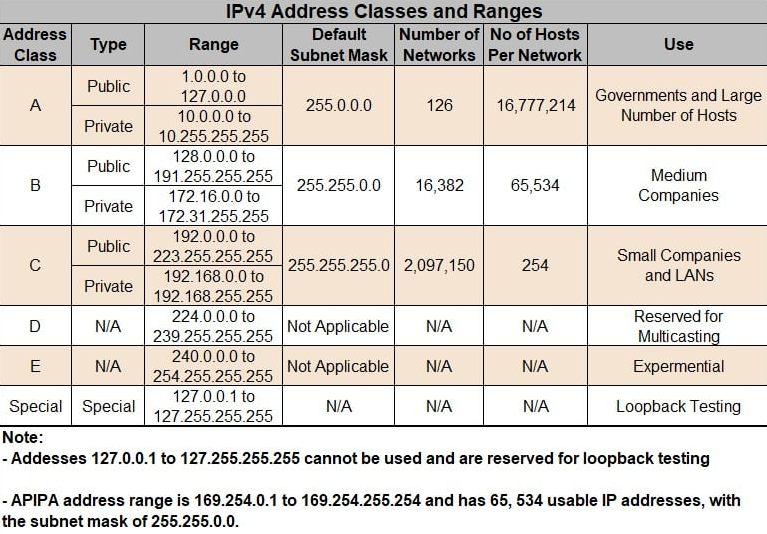
\includegraphics[width=0.8\textwidth]{images/ip_addresses.png}
    \caption{IP addresses types.}
    \label{fig:ip_address}
\end{figure}
